


\chapter{State-space Covariates}
\markboth{Chapter 9 }{}
\label{chapt.state-space}

\vspace{0.3cm}

Underlying all spatial capture recapture models is a point process
model describing the distribution of individual activity
centers (${\bf s}_i$) within the state space ($\cal{S}$). So far we have focused our
discussion on the homogeneous binomial point process,
${\bf s}_i \sim Uniform({\cal S}), i=1,2,\dots,N$, where $N$ is the
size of the population. This is a model of
``spatial-randomness''\footnote{The phrase ``complete
  spatial-randomness'' is reserved for the homogeneous Poisson point
  process}
because the intensity of the
activity centers is constant across the study area and the activity
centers are distributed independently of each other.

The spatial-randomness assumption is often viewed as restrictive
because ecological processes such as
territoriality and habitat selection can result in non-random
distributions of organisms. We have argued, however, that this
assumption is less restrictive than may be recognized because the
homogeneous point process actually allows for infinite
possible configurations of activity centers. Furthermore, given enough data,
the uniform prior will have very little influence on the estimated
locations of activity centers. Nonetheless, the homogeneous point
process model does not allow one to model population density using
covariates---a central objective of much ecological research.
For example, a homogeneous point process model
may result in a density surface map indicating that individuals were
more abundant in one habitat than another, but it does not do so
explicitly. A more direct approach would be to model density using
covariates as is done in generalized linear models (GLMs)
\citep{mccullagh_nelder:1989}. % where a
%link function is used to connect the intensity parameter to the linear
%predictor.

In this chapter we will present a method
for fitting inhomogeneous binomial point process models using
covariates in much the same way as is done with GLMs. The
covariates we consider differ
from those covered in previous chapters, which were typically
attributes of the animal ({\it e.g.} sex or age) and were used to model movement or encounter
rate. In contrast, here we wish to
model covariates that are defined for all points in
$\cal{S}$, which we will refer to as
state-space, or density, covariates. These may
include continuous covariates such as elevation, or discrete
covariates such as habitat type.

\citet{borchers_efford:2008} were the first to propose an
inhomogeneous point process model for SCR models, and our approach is
similar to theirs with the exception that we will use a binomial
rather than a Poisson model because the binomial model is
easily integrated into our data augmentation scheme and is consistent
with the objective of determining how a {\it fixed} number of activity
centers are distributed with respect to covariates.

The method we use to accommodate inhomogeneous binomial point process
models within our MCMC algorithm is simple---we
replace the uniform prior with a prior describing the
distribution of the $N$ activity centers conditional on the
covariates. Development of this prior, which does not have a
standard form, is a central component of this chapter. First we will
begin with a review of homogeneous point process models.


\section{Homogeneous point process revisited}

The homogeneous Poisson point process is \emph{the} model of ``complete
spatial randomness'' and is often used in ecology as a null model
to test for departures from randomness
\citep{diggle:2003,illian_etal:2008}. Given its central role in the
analysis of point procesess, it is helpful to compare it with
the binomial model that we use in our SCR models. The
primary descriptor of the homogeneous point process model is the
``intensity'' parameter, $\mu$ which describles the expected number
of points in an infinitesimally small area. The intensity
parameter can also be used to determine the expected number of points
in any region $B$ of the state-space $\cal{S}$. To denote this, we say
that the expected number of points in region $B \in \cal{S}$ is
$\mathbb{E}[n(B)] = A(B)\mu$ where $A(B)$ is the area of region $B$.  In words,
the expected number of points in $B$ is simply the area of $B$
muliplied by the intensity parameter. One property
of the Poisson model is that if we divide the entire state-space into
$k=1,\dots,K$ disjunct regions, the counts $\bf n(B)$ are
independent and identically distributed, ({\it i.i.d.}). This is one
of the distinctions between the Poisson model and the binomial model,
for which the counts $n(B_k)$ are not {\it i.i.d.} as we will explain
shortly. This difference is also related to another distinction
between the two models, namely that the binomial model
conditions on the number of points to be simulated $N$; whereas under
the Poisson model $N$ is random. Here is some simple \R~code to
illustrate this point.

\begin{center} % doesn't work
\begin{verbatim}
mu <- 4                            # intensity
Np <- rpois(1, mu)                 # Np is random
PPP <- cbind(runif(Np), runif(Np)) # Poisson point process

Nb <- 4                            # Nb is fixed
BPP <- cbind(runif(Nb), runif(Nb)) # Binomial point process
\end{verbatim}
\end{center}

Note that in both models, the $N$ points are independent
of one another and distributed uniformly
throughout $\mathcal{S}$. Thus, the intensity at any point $x \in
\cal{S}$ is $\mu = 1 / A(\mathcal{S})$ where $A(\mathcal{S})$ denotes
the area of the state-space. In the \R~code above, the area of the
state-space is 1 unit, and thus the intensity is $\mu = 1/1$.

Although the Poisson model is typically described in terms of $\mu$,
the binomial model is not; rather, it
is more common to consider a discrete state space, such as a grid with
with $K$ pixels. Under the binomial model, the number of points in
each region is $n(B_k) \sim Bin(N, p_k)$
where $p_k = A(B)/A(\cal{S})$, ie $p_k$ is simply the fraction of
the state-space area in $B_k$. This discrete space representation of
the binomial point process is shown in Fig.~\ref{ch9.fig.homo}. The
state-space in this case is the unit square, and thus the probability of a
point falling in each of the 25 disjunct regions is $p_k = 1/25$ and
thus the expected counts are simply $\mathbb{E}(n(B_k)) = Np_k$. In
the figure $N=50$ and thus we would expect 2 points per pixel, which
happens to be the empirical mean of the data in
Fig.~\ref{ch9.fig.homo}. Note also that these counts are not
independent realizations from a binomial distribution since $\sum_k
n(B_k) = N$. Instead, the model for the entire vector
is ${\bf n(B)} \sim Multinomial(N, {\mathbf{\pi}} = (p_1, p_2, \dots,
p_K))$ \citep{illian_etal:2008}. The dependence among counts has virtually
no practical consequence when the number of pixels is large. For
example, if we have 100 pixels, the number of points in one pixels
tells you very little about the expected number of points in another
pixel. However, if there are only 2 pixels, then clearly the number of
points in one pixel tells you exactly how many will occur in the
remaining pixel. To gain familiarity with the multinomial distribution
and the discrete representation of space, use the \verb+rmultinom+
function in \R~to simulate counts similar to those shown in
Fig.~\ref{ch9.fig.homo}, for example using a command
such as:

\begin{verbatim}
n.B_k <- rmultinom(1, size=50, prob=rep(1/25, 25))
matrix(n.B_k, 5, 5)
\end{verbatim}


\begin{figure}
\centering
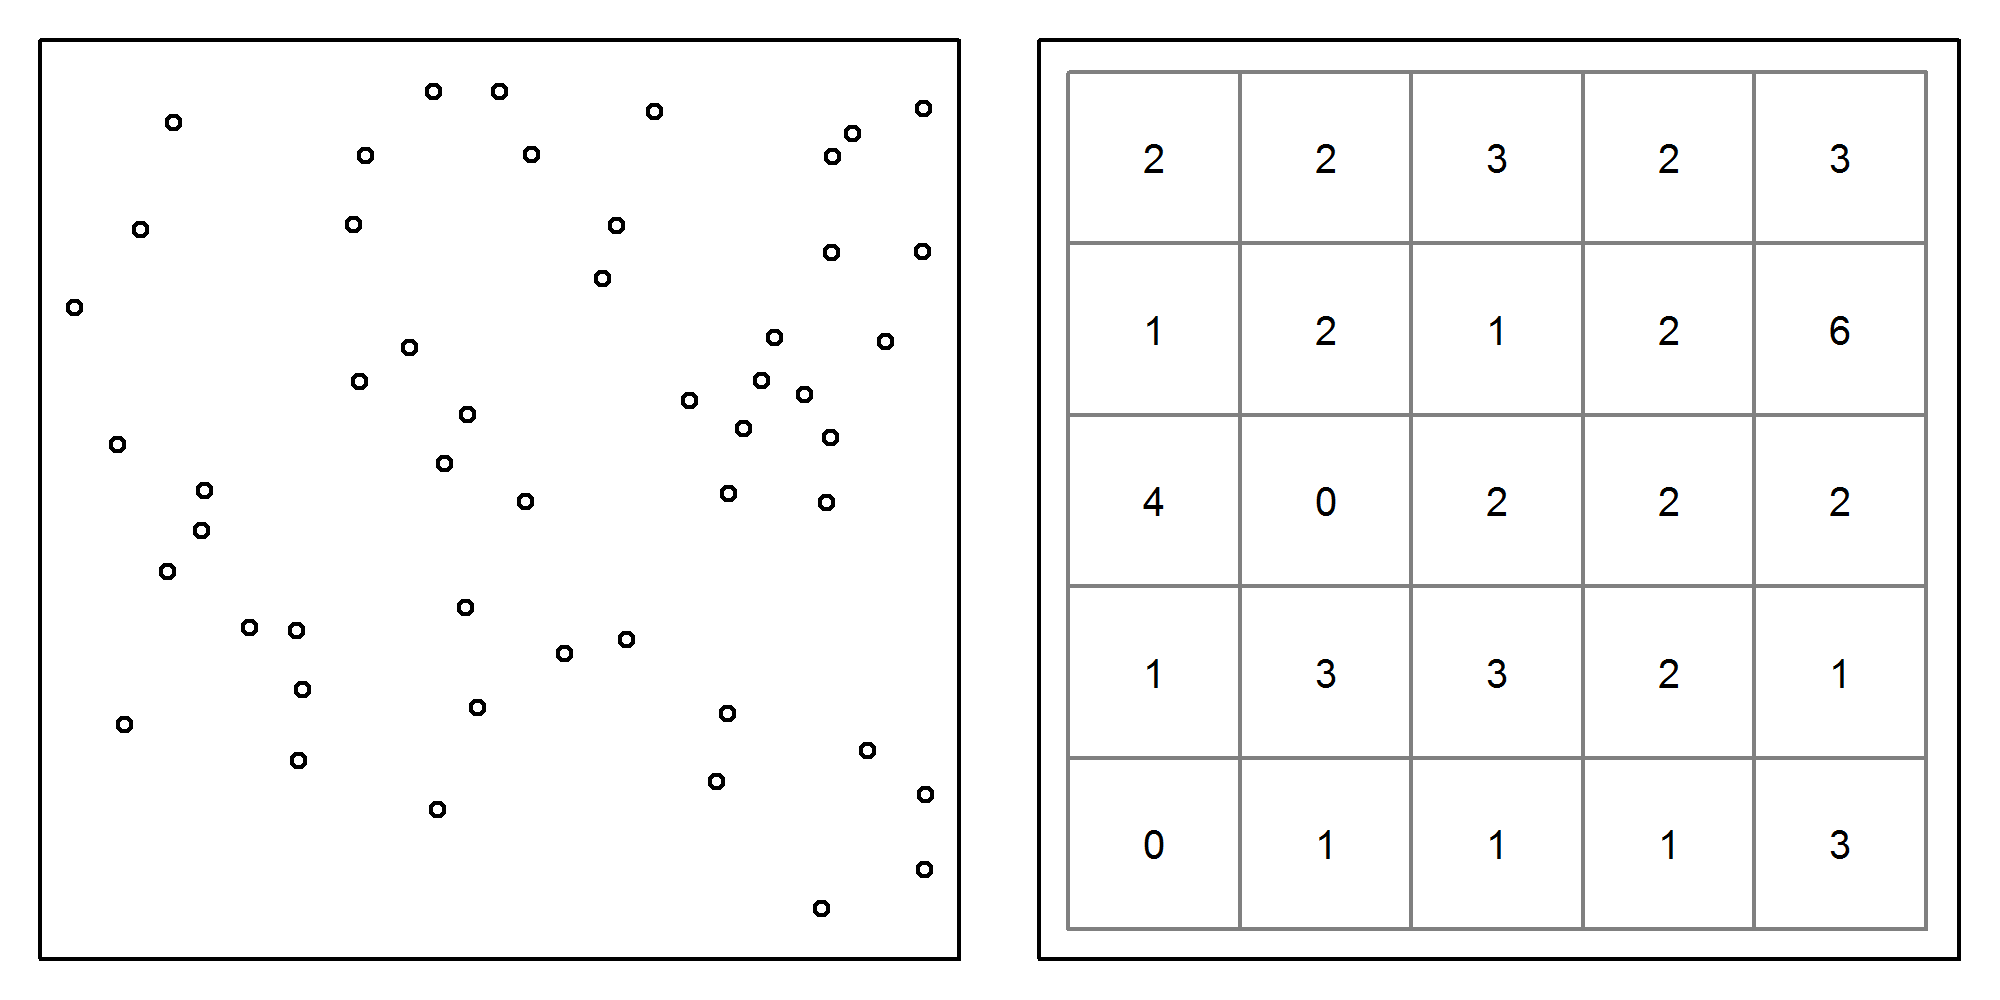
\includegraphics[width=5in,height=2.5in]{Ch11/figs/homoPlots}
\label{ch9.fig.homo}
\caption{Homogeneous binomial point process with $N$=50 points
  represented in continuous and discrete space.}
\end{figure}


The discrete space representation of the binomial point process is of
practical importance when fitting SCR models because spatial covariates
are almost always represented in a discrete format, often called
``rasters'' in GIS-speak. In such cases, we often need to change our
definition of the prior for an activity center from $s_i \sim
Uniform(\cal{S})$ to $s_i \sim Multinomial(1, \mathbf{\pi})$. In the
latter case, the activity center is simply defined as an integer
representing pixel ``id''. Note also that the multinomial distribution
with an index of 1 (\emph{i.e.} \verb+size=1+ in \verb+rmultinom+)
is referred to as the categorical distribution,
which we will frequently use in the \verb+BUGS+ language.



\section{Inhomogeneous binomial point process}

As with the homogeneous model, the inhomogeneous binomial point process
model is developed conditional on $N$. The primary distinction is that
the uniform distribution is replaced with another distribution
allowing for the intensity parameter to vary spatially. To arrive at
this new distribution, define $\mu(x, {\bf \beta})$ to be a function of
spatially-referenced covariates ($\mathbf{v(x)}$) available at all points of the state
space.  To be concise we will subsequently drop the vector of cofficients from our
notation, and simply use $\mu(x)$. Since an intensity must be strictly
positive, it is natural to model $\mu(x)$ using the log-link.
\[
\log(\mu(x)) = \sum_{j=1}^J \beta_j v_j(x), \quad  x \in \cal{S}
\]
where $\beta_j$ is the regression coefficient for covariate
$v_j(x)$. To be clear, $v(x)$ is the value of any covariate, such as
habitat type or elevation, at location $x$.  This equation should look
familiar because it is the standard linear model used in log-linear
GLMs. Note, however, that we have no need
for an intercept because it would be confounded with
$N$. This should be intuitive since an intercept would
represent the expected value of $N$ when $\beta=0$, but we already
have a parameter in the model for expected abundance, namely $\mathbb{E}[N] =
\psi M$. Thus an intercept would be
redundant, and without it we are still able to achieve our goal of
describing the distribution of $N$ activity centers as a function of
spatial covariates.

Now that we have a model of the intensity parameter $\mu(x)$,
we need to develop the associated probability density function to use
in place of the uniform prior. Remembering that
the integral of a pdf must be unity, we can create a pdf by dividing
$\mu(x)$ by a normalizing constant, which in this case is the integral
of $\mu(x)$ evlauated over the entire
state-space\hl{ANDY, is there a better justification for this?}. The
probability density function is therefore
\begin{equation}
f(x) = \frac{\mu(x)}{\int_{x \in \mathcal{S}} \mu(x)\, \mathrm{d}x}
\label{eq:pdf-ipp}
\end{equation}
Substituting this distribution for the
uniform prior allows us to fit inhomogeneous binomial point process
models to spatial capture-recapture data. We can also use this
distribution to obtain the expected number of individuals in any given
region. Specifically, the proportion of $N$ expected to occur in any
region $B$ when heterogeneity in density is present is $p(B) = \int_B
f(x)\, \mathrm{d}x$. These are
also the multinomial cell probabilities if the regions are
disjoint and compose the entire state-space.

As a practical matter, note that the integral in the
demoninator of $f(x)$ is evaluated over space, and since we always regard
space as two-dimensional, this is a two-dimensional integral that can
be approximated using the methods discussed in
Chapter~\ref{chapt.poisson-mn}. These methods include
Monte Carlo integration, Gaussian quadrature, etc... Alternatively, if
our state-space covariates are in raster format, \emph{i.e} they are
in discrete space, the integral can be replaced with a sum over
all pixels, which is much more efficient computationally.

We now have all the tools needed to fit inhomogeneous point process
(IPP) models. Before doing so, we note that the IPP for the activity centers
results in another IPP for the observation process, $\lambda(x)$. As
a reminder, $\lambda(x)$ is the expected number of captures for a trap
at point $x$. As was true for the homogeneous model, this
intensity function is a product of the point process intensity
and the encounter rate function, $\lambda(x) = \mu(x) g(x)$.

In the next section we walk through a few examples, building up from
the simplest case where we actually observe the activity centers as
though they were data. In the second example, we fit our new model to simulated
data in which density is a function of a single continuous
covariate. Example three shows an analysis in discrete space using
both \secr~\citep{efford:2011} and \jags~\citep{plummer:2003}. In the
last example, we model the intensity of
activity centers for a real dataset collected on jaguars
(\emph{Panthera onca}) in Argentina.

\section{Examples}

\subsection{Simulation and analysis of inhomogeneous point processes}

In SCR models, the point process is not directly observed, but in
other contexts it is. Examples include the locations of disease
outbreaks, the locations of trees in a forest, or the locations of
radio-tracked animals. Indeed Eq.~\ref{eq:pdf-ipp} has been used
extensively in the radio-telemetry literature to model so-called
``resource selection functions'' \citep{manly:2002,lele_keim:2006}.
In such cases where the point locations are directly observed,
estimating the parameters $\bf \beta$ is straight-forward as
demonstrated in the following example. This example also illustrates
the fundamental process that we will later embed in our MCMC algorithm
used to fit SCR models.

Suppose we knew the locations of 100 animals' activity
centers. To estimate the intensity surface $\mu(x)$ underlying these points, we
need to derive the likelihood for our data under this model. Given the
pdf $f(x)$ (Eq.~\ref{eq:pdf-ipp}) and assuming that the points are
mutually independent of one another,
the likelihood is given by the product
of $R$ such terms, where $R=100$ is the sample size in this case,
\emph{ie} the observed number of activity centers.
\[
\mathcal{L}({\bf \beta} | {\bf x}_i) = \prod_{i=1}^R f(x_i)
\]
Having defined the likelihood we could choose a prior and obtain the posterior for
$\bf \beta$ using Bayesian methods, or we can find the maximum likelihood
estimates (MLEs) using standard numerical methods as is demonstrated
below.

First, let's simulate some data. Simulating data under an inhomogeneous point process model is often
accomplished using indirect methods such as rejection
sampling. Rejection sampling proceeds by
simulating data from a standard distribution and then accepting or
rejecting each sample using probabilities defined by the distribution
of interest. For more information, readers should consult an
accessible text such as \citet{robert_casella:2004}. In our example, we
simulate from a uniform distribution and then accept or reject using
the (scaled) probability density function $f(x)$. Note that we first define a
spatial covariate (elevation) that is a simple function of the spatial
coordinates increasing from the southwest to the northeast of our
state-space.\footnote{Such functional forms of
covariates are rarely available, which is why continuous spatial
covariates are more often measured on a discrete grid.}

The following \R~commands demonstrate the use of rejection sampling to
simulate an inhomogeneous point process for the covariate depicted in
Fig.~\ref{ch9:fig:hetero}. The code uses the \verb+cuhre+ function in
the {\tt R2Cuba} package to integrate the intensity function over
space \citep{hahn_etal:2011}.

\begin{small}
\begin{verbatim}
# spatial covariate (with mean 0)
elev.fn <- function(x) x[1]+x[2]-1
# intensity function
mu <- function(x, beta) exp(beta*elev.fn(x=x))

# Simulate PP using rejection sampling
set.seed(300225)
N <- 100
count <- 1
s <- matrix(NA, N, 2)
beta <- 2 # parameter of interest
int.mu <- R2Cuba:::cuhre(2, 1, mu, beta=beta)$value
elev.min <- elev.fn(c(0,0)) #elev.fn(cbind(0,0))
elev.max <- elev.fn(c(1,1)) #elev.fn(cbind(1,1))
Q <- max(c(exp(beta*elev.min) / int.mu,   #2d(beta),
           exp(beta*elev.max) / int.mu))   #2d(beta)))
while(count <= 100) {
  x.c <- runif(1, 0, 1); y.c <- runif(1, 0, 1)
  s.cand <- c(x.c,y.c)
  pr <- exp(beta*elev.fn(s.cand)) / int.mu #2d(beta)
  if(runif(1) < pr/Q) {
    s[count,] <- s.cand
    count <- count+1
    }
  }
\end{verbatim}
\end{small}


\begin{figure}
\centering
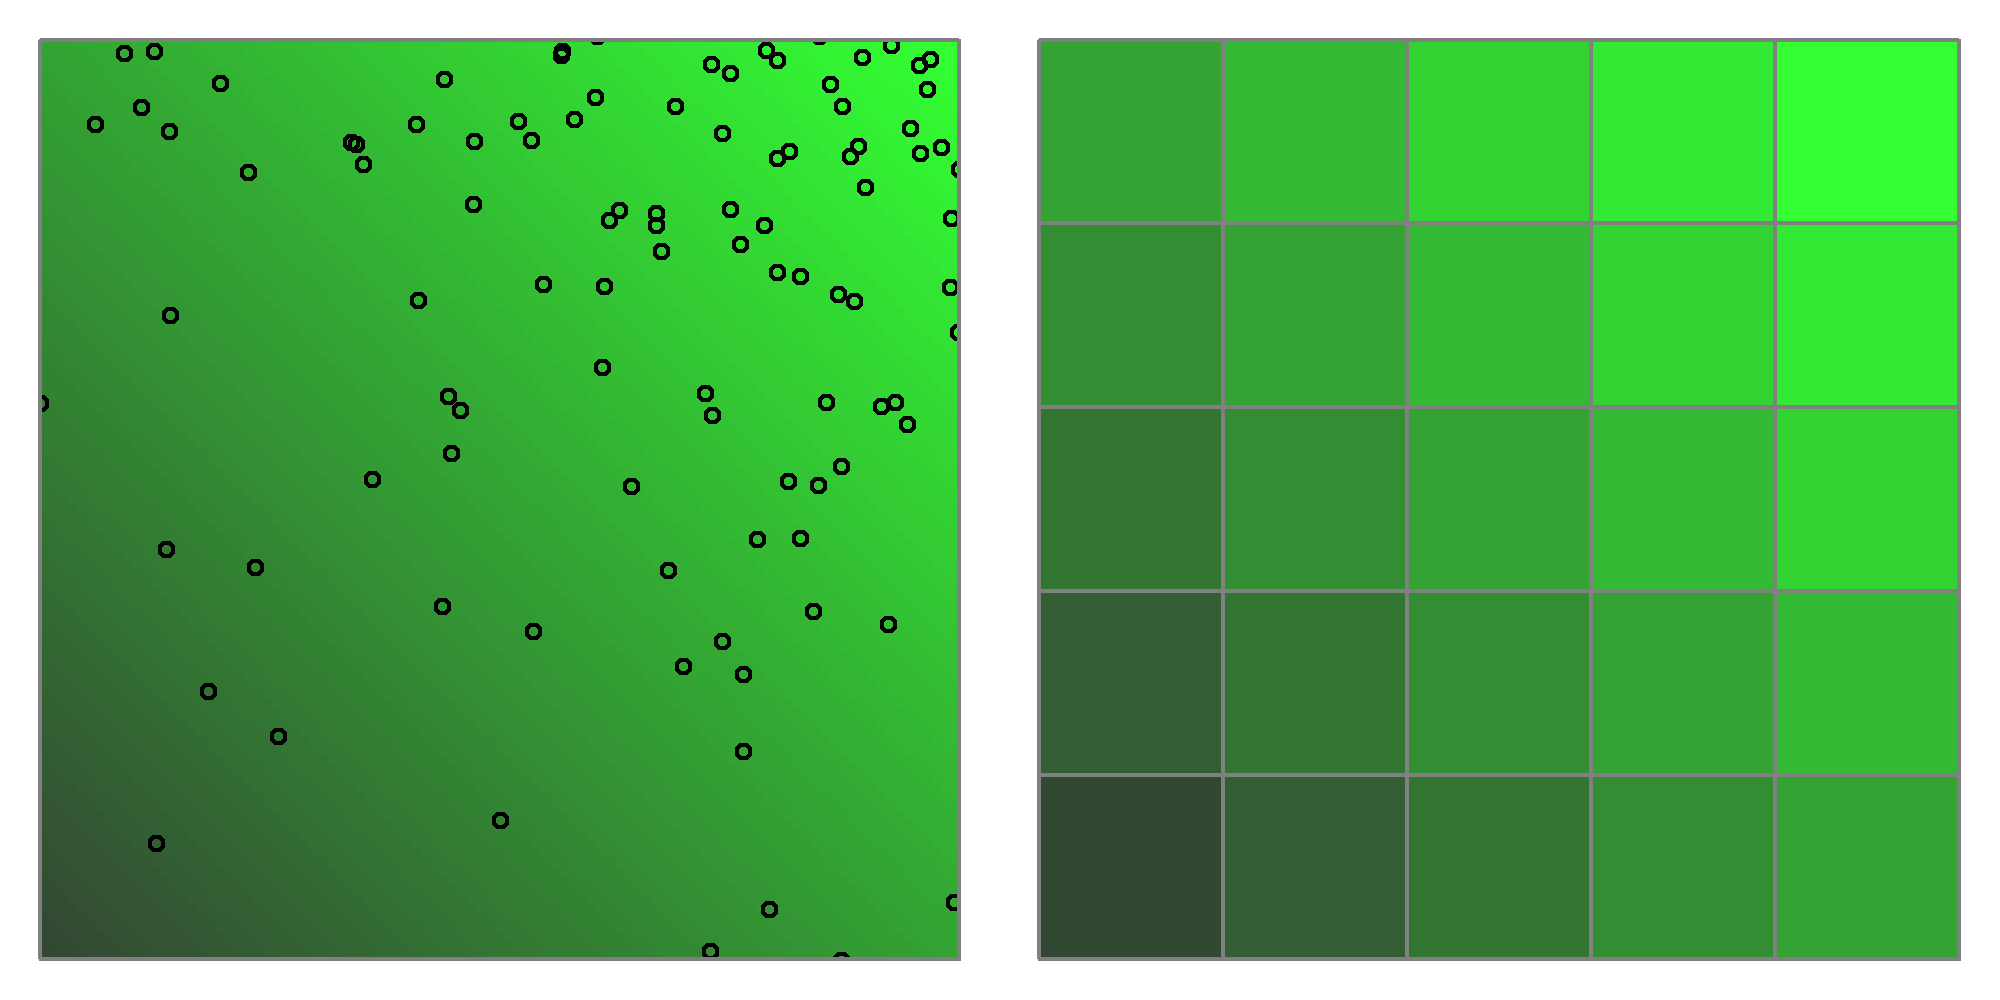
\includegraphics[width=5in,height=2.5in]{Ch11/figs/heteroPlots}
\label{ch9:fig:hetero}
\caption{An example of a spatial covariate, say elevation, and a
  realization of a inhomogeneous binomial point process with $N$=100
  and $\mu(x) = exp(\beta Elev)$ where $\beta=2$.}
\end{figure}

The simulated data are shown in Fig~\ref{ch9:fig:hetero}. High elevations
are represented by light green and low elevations by dark green. The
activity centers of one hundred animals are shown as
points, and it is clear that these simulated animals prefer the high
elevations.  Perhaps they are mountain goats. The underlying model describing this preference is
$\log(\mu(x)) = exp(\beta \times Elevation(x))$
where $\beta=2$ is the parameter to be estimated and $Elevation(x)$
is a function of the coordinates at $x$, as displayed on the map.

Given these points, we will now estimate $\beta$ by minimizing the
negative-log-likelihood using \verb+R+'s \verb+optim+ function.

\begin{small}
\begin{verbatim}
# Negative log-likelihood
nll <- function(beta) {
    int.mu <- cuhre(2, 1, mu, beta=beta)$value
    -sum(beta*elev.fn(s) - log(int.mu))
}
starting.value <- 0
fm <- optim(starting.value, nll, method="Brent",
            lower=-5, upper=5, hessian=TRUE)
c(Est=fm$par, SE=sqrt(1/fm$hessian)) # estimates and SEs
\end{verbatim}
\end{small}


Maximizing the likelihood took a small fraction of a second, and we
obtained an estimate of $\hat{\beta}=1.99$. We could plug
this estimate into our linear model at each point in the state-space to
obtain the MLE for the intensity surface.

This example demonstrates
that if we had the data we wish we had, {\it i.e.} if we knew the
coordinates of the activity centers, we could easily estimate the
parameters governing the underlying point process. Unfortunately, in
SCR models, the activity centers cannot be directly observed, but
spatial re-captures, that is captures of individuals at
multiple locations in space, provide us with the information needed to
estimate these latent parameters.

\subsection{Fitting inhomogeneous point process SCR models}

\subsubsection{Continuous space}

One of the nice things about hierarchical models is that they allow us
to break a problem up into a series of simple conditional
relationships. Thus,
we can simply add the methods described above into our existing MCMC
algorithm to simulate the posteriors of $\beta$ conditional on the
simulated values of $\mathbf{s}_i$. To demonstrate, we will continue with
the previous example. Specifically, we will overlay a grid of
traps upon the map shown in Fig.~\ref{ch9:fig:hetero}. We will then
simulate capture histories conditional upon the activity centers shown
on the map. Then, we will attempt to estimate the activity center
locations as though we did not know where they were, as is the case in
real applications.

Here is some \R~code to simulate the encounter histories under a
Poisson observation model, which would be appropriate if animals could
be detected multiple times at a trap during a single occassion.

\begin{small}
\begin{verbatim}
# Create trap locations
xsp <- seq(-0.8, 0.8, by=0.2)
len <- length(xsp)
X <- cbind(rep(xsp, each=len), rep(xsp, times=len))

# Simulate capture histories, and augment the data
ntraps <- nrow(X)
T <- 5
y <- array(NA, c(N, ntraps, T))

nz <- 50 # augmentation
M <- nz+nrow(y)
yz <- array(0, c(M, ntraps, T))

sigma <- 0.1  # half-normal scale parameter
lam0 <- 0.5   # basal encounter rate
lam <- matrix(NA, N, ntraps)

set.seed(5588)
for(i in 1:N) {
    for(j in 1:ntraps) {
        distSq <- (s[i,1]-X[j,1])^2 + (s[i,2] - X[j,2])^2
        lam[i,j] <- exp(-distSq/(2*sigma^2)) * lam0
        y[i,j,] <- rpois(T, lam[i,j])
    }
}
yz[1:nrow(y),,] <- y # Fill
\end{verbatim}
\end{small}

Now that we have a simulated capture-recapture dataset $y$, and we have
augmented it to create the new data object $yz$, we are ready to
begin sampling from the posteriors. A commented Gibbs sampler written
in \R~is available in the accompanying \R~package \scrbook~(see
?scrIPP). There are two small parts of the
\R~code that distinguish it from previous code we have shown to
fit homogeneous point processes. First, we need to update the parameter
${\bf \beta}$ conditional on all other parameters in the model. The code to
do so is:

\begin{small}
\begin{verbatim}
D1 <- cuhre(2, 1, mu, lower=c(xlims[1], ylims[1]),
            upper=c(xlims[2], ylims[2]), beta=beta1)$value
beta1.cand <- rnorm(1, beta1, tune[3])
D1.cand <- cuhre(2, 1, mu, lower=c(xlims[1], ylims[1]),
                 upper=c(xlims[2], ylims[2]), beta=beta1.cand)$value
ll.beta1 <- sum(  beta1*elev.fn.v(S) - log(D1) )
ll.beta1.cand <- sum( beta1.cand*elev.fn.v(S) - log(D1.cand) )
if(runif(1) < exp(ll.beta1.cand - ll.beta1) )  {
     beta1<-beta1.cand
}
\end{verbatim}
\end{small}

Next, we need to put the new prior on the activity centers:

\begin{small}
\begin{verbatim}
#ln(prior), denominator is constant
prior.S <- beta1*cov(S[i,1], S[i,2]) # - log(D1)
prior.S.cand <- beta1*(Scand[1] + Scand[2]) # - log(D1)
if(runif(1)< exp((ll.S.cand+prior.S.cand) - (ll.S+prior.S))) {
    S[i,] <- Scand
    lam <- lam.cand
    D[i,] <- dtmp
    }
\end{verbatim}
\end{small}

We can apply this modified sampler to our data using the code shown in
the help file for \verb+scrIPP+. We obtain posterior
distributions summarized in Table~\ref{ch9:tab:simIPP}. Mixing is good, and as usual,
life is very nice when we are working with simulated data.

\begin{table}[b]
\centering
\caption{Posterior summaries from inhomogeneous point proces model}
\begin{tabular}{lrrrrr}
\hline
& Mean & SD & 2.5\% & 50\% & 97.5\% \\
\hline
 $\sigma =0.10$ &   0.1026 &   0.0048 &   0.0935 &   0.1025 &   0.1123 \\
 $\lambda_0=0.50$ &   0.4419 &   0.0493 &   0.3496 &   0.4400 &   0.5390 \\
 $\psi =0.66$ &   0.6826 &   0.0554 &   0.5762 &   0.6820 &   0.7923 \\
 $\beta =2.00$ &   2.1601 &   0.3390 &   1.5193 &   2.1583 &   2.8043 \\
 $N =100$ & 102.7696 &   6.2689 &  92.0000 & 102.0000 & 117.0000 \\
\hline
\end{tabular}
\label{ch9:tab:simIPP}
\end{table}


Fitting continuous space IPP models is somewhat
difficult in \bugs~because our prior $f(x)$ is not one of the
available distributions that come with the software\footnote{It is
  possible, if somewhat
  cumerbersome, to add new distributions in \bugs.} \secr~allows
users to fit continuous space using polynomials of the x- and y-
coordinates, but not for truly continuous covariates. However, these
are not really important limitations because discrete
space versions are straight-forward, and virtually all spatial
covariates are defined as such.


\subsubsection{Discrete space}

To fit discrete space models, we follow the same steps
as outlined in Chapter XXX---we define $s_i$ as
pixel ID, and we use the categorical distribution as a prior. A good
example of this is in +cite{Kery capricaillie}. Here we present
an analysis of the simulated data shown in the right panel of
Fig.~\ref{ch9:fig:hetero}. The spatial covariate, let's call it
elevation again, was simulated
from a kriging type of model as shown on the help page
\verb+ch9simData+ in \scrbook. The points are the number of
activity centers in each pixel, generated from a single realization of
the IPP $mu(x) = 2elev$.


\begin{figure}
\centering
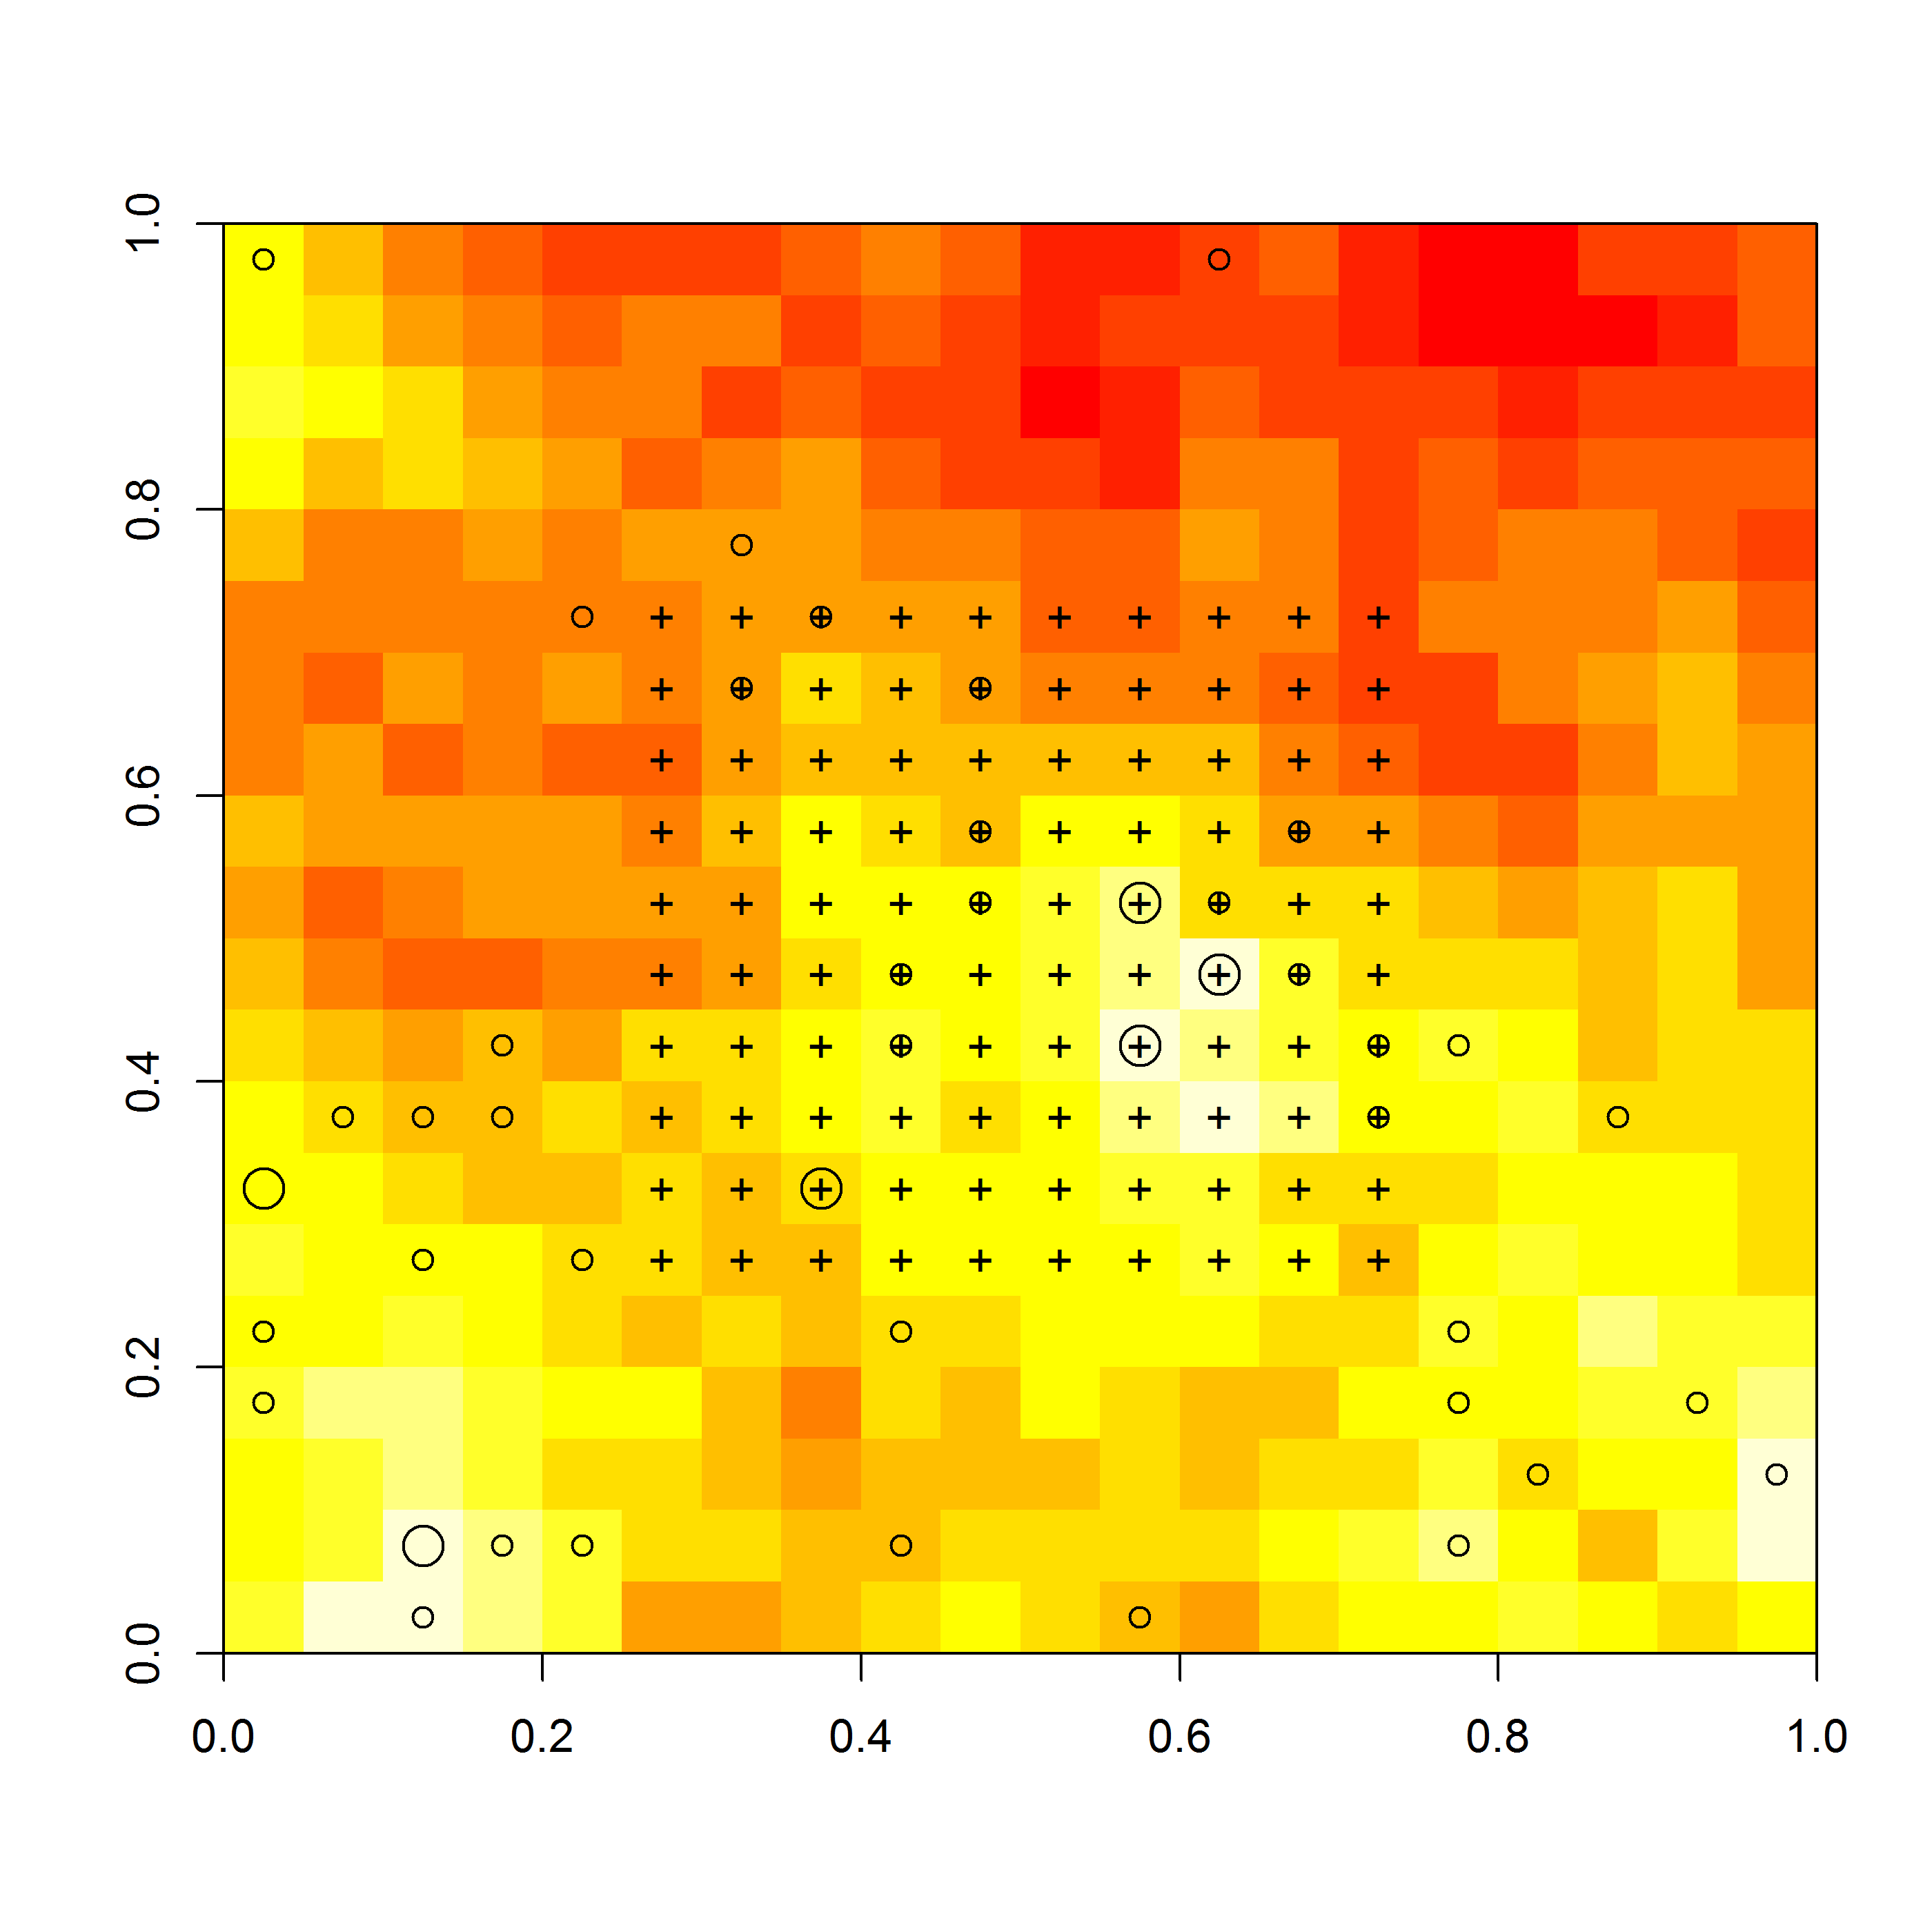
\includegraphics[width=3in,height=3in]{Ch11/figs/discrete}
\label{ch9:fig:discrete}
\caption{Simulated activity centers in discrete space. The spatial
  covariate, elevation, is highest in the ligher areas. Density of
  activity centers (circles) increases with elevation. Trap locations
  are shown as crosses.}
\end{figure}


The \bugs~code to fit an IPP model to these data is shown in
the following panel.

\begin{small}
\begin{verbatim}
model{
sigma ~ dunif(0, 1)
lam0 ~ dunif(0, 5)
beta ~ dnorm(0,0.1)
psi ~ dbeta(1,1)

for(j in 1:nPix) {
  theta[j] <- exp(beta*elevation[j])
  probs[j] <- theta[j]/sum(theta[])
}

for(i in 1:M) {
  w[i] ~ dbern(psi)
  s[i] ~ dcat(probs[])
  x0g[i] <- Sgrid[s[i],1]
  y0g[i] <- Sgrid[s[i],2]
  for(j in 1:ntraps) {
    dist[i,j] <- sqrt(pow(x0g[i]-grid[j,1],2) + pow(y0g[i]-grid[j,2],2))
    lambda[i,j] <- lam0*exp(-dist[i,j]*dist[i,j]/(2*sigma*sigma)) * w[i]
    y[i,j] ~ dpois(lambda[i,j])
    }
  }

N <- sum(w[])
Density <- N/1 # unit square
}
\end{verbatim}
\end{small}


\begin{table}[b]
\centering
\caption{Comparision of \secr~and \jags~results}
\begin{tabular}{llrrrr}
\hline
Software & Par & Est. & SD & lower & upper \\
\hline
 secr & $N$ & 49.2803 & 5.7535 & 41.0087 & 64.3879 \\
      & $\beta$ &  2.1772 & 0.5628 &  1.0741 &  3.2804 \\
      & $\lambda_0$ &  0.9203 & 0.0764 &  0.7824 &  1.0825 \\
      & $\sigma$ &  0.0990 & 0.0038 &  0.0918 &  0.1068 \\
 JAGS & $N$ & 48.2072 & 5.4053 & 39.0000 & 60.0000 \\
      & $\beta$ &  2.1026 & 0.5323 &  1.0889 &  3.1506 \\
      & $\lambda_0$ &  0.9328 & 0.0766 &  0.7898 &  1.0921 \\
      & $\sigma$ &  0.1004 & 0.0041 &  0.0929 &  0.1089 \\
\hline
\end{tabular}
\label{ch9:tab:secrYjags}
\end{table}


This model can also be fit in \secr, which refers
to the pixel locations as a ``mask''. \R~code to
fit the models using \secr~and \jags~is available in \scrbook~, see
\verb#help(ch9secrYjags)#. Results of the
comparision are shown in Table \ref{ch9:tab:secrYjags} and are
very similar as expected.

Density surface maps can be created for fun, and of course to inform
management decisions. [describe how to do this]


\subsection{The jaguar data}

Estimating density of large felines has been a priority for many
conservation organizations, but no robust methodologies existed before
the advent of SCR. Distance sampling is not feasible for such rare and
cryptic species, and traditional capture-recapture methods yield
estimates that are highly sensitive to the subjective choice of the
effective survey area. In this example, we
demonstrate how readily density can be estimated for a
globally imperilled species using SCR. Furthermore, we show how
inhomogeneous point process models can be used to test important
hypotheses regarding the factors affecting density.

In this example, we make use a single year of data from an 8-year
camera-trapping study of jaguars (\emph{Panthera onca}) in Argentina,
along the borders with Brazil and Paraguay. The data consist of 46
camera stations, each consisting of a camera on either side of a
road or trail. Forty-five detections of 16 jaguars were made over a 95
day sampling period. The mean number of sampling days at each camera
station was 48.2. Eight females and 8 males were detected.

Estimating density is a central objective of this study because
ultimately, an estimate of the total population size for the ``green
corridor'' is needed. A second, and related, objective was to assess
the influence of poaching on jaguar density. Although jaguars
themselves are occasionally killed by poachers, the bigger influence
is the effect of poaching on prey species such as peccaries
(\emph{Pecari tajacu, Tayassu pecari} ASK AGUSTIN WHICH ARE MORE
COMMON). To protect jaguars and related species, protected areas have
been established (DETAILS) and three levels of protection are
recognized as depicted in Fig.~\ref{ch9:fig:jaguarCts}.

MENTION SEX-SPECIFIC SIGMAS

MENTION THE RIVER

\begin{figure}
\centering
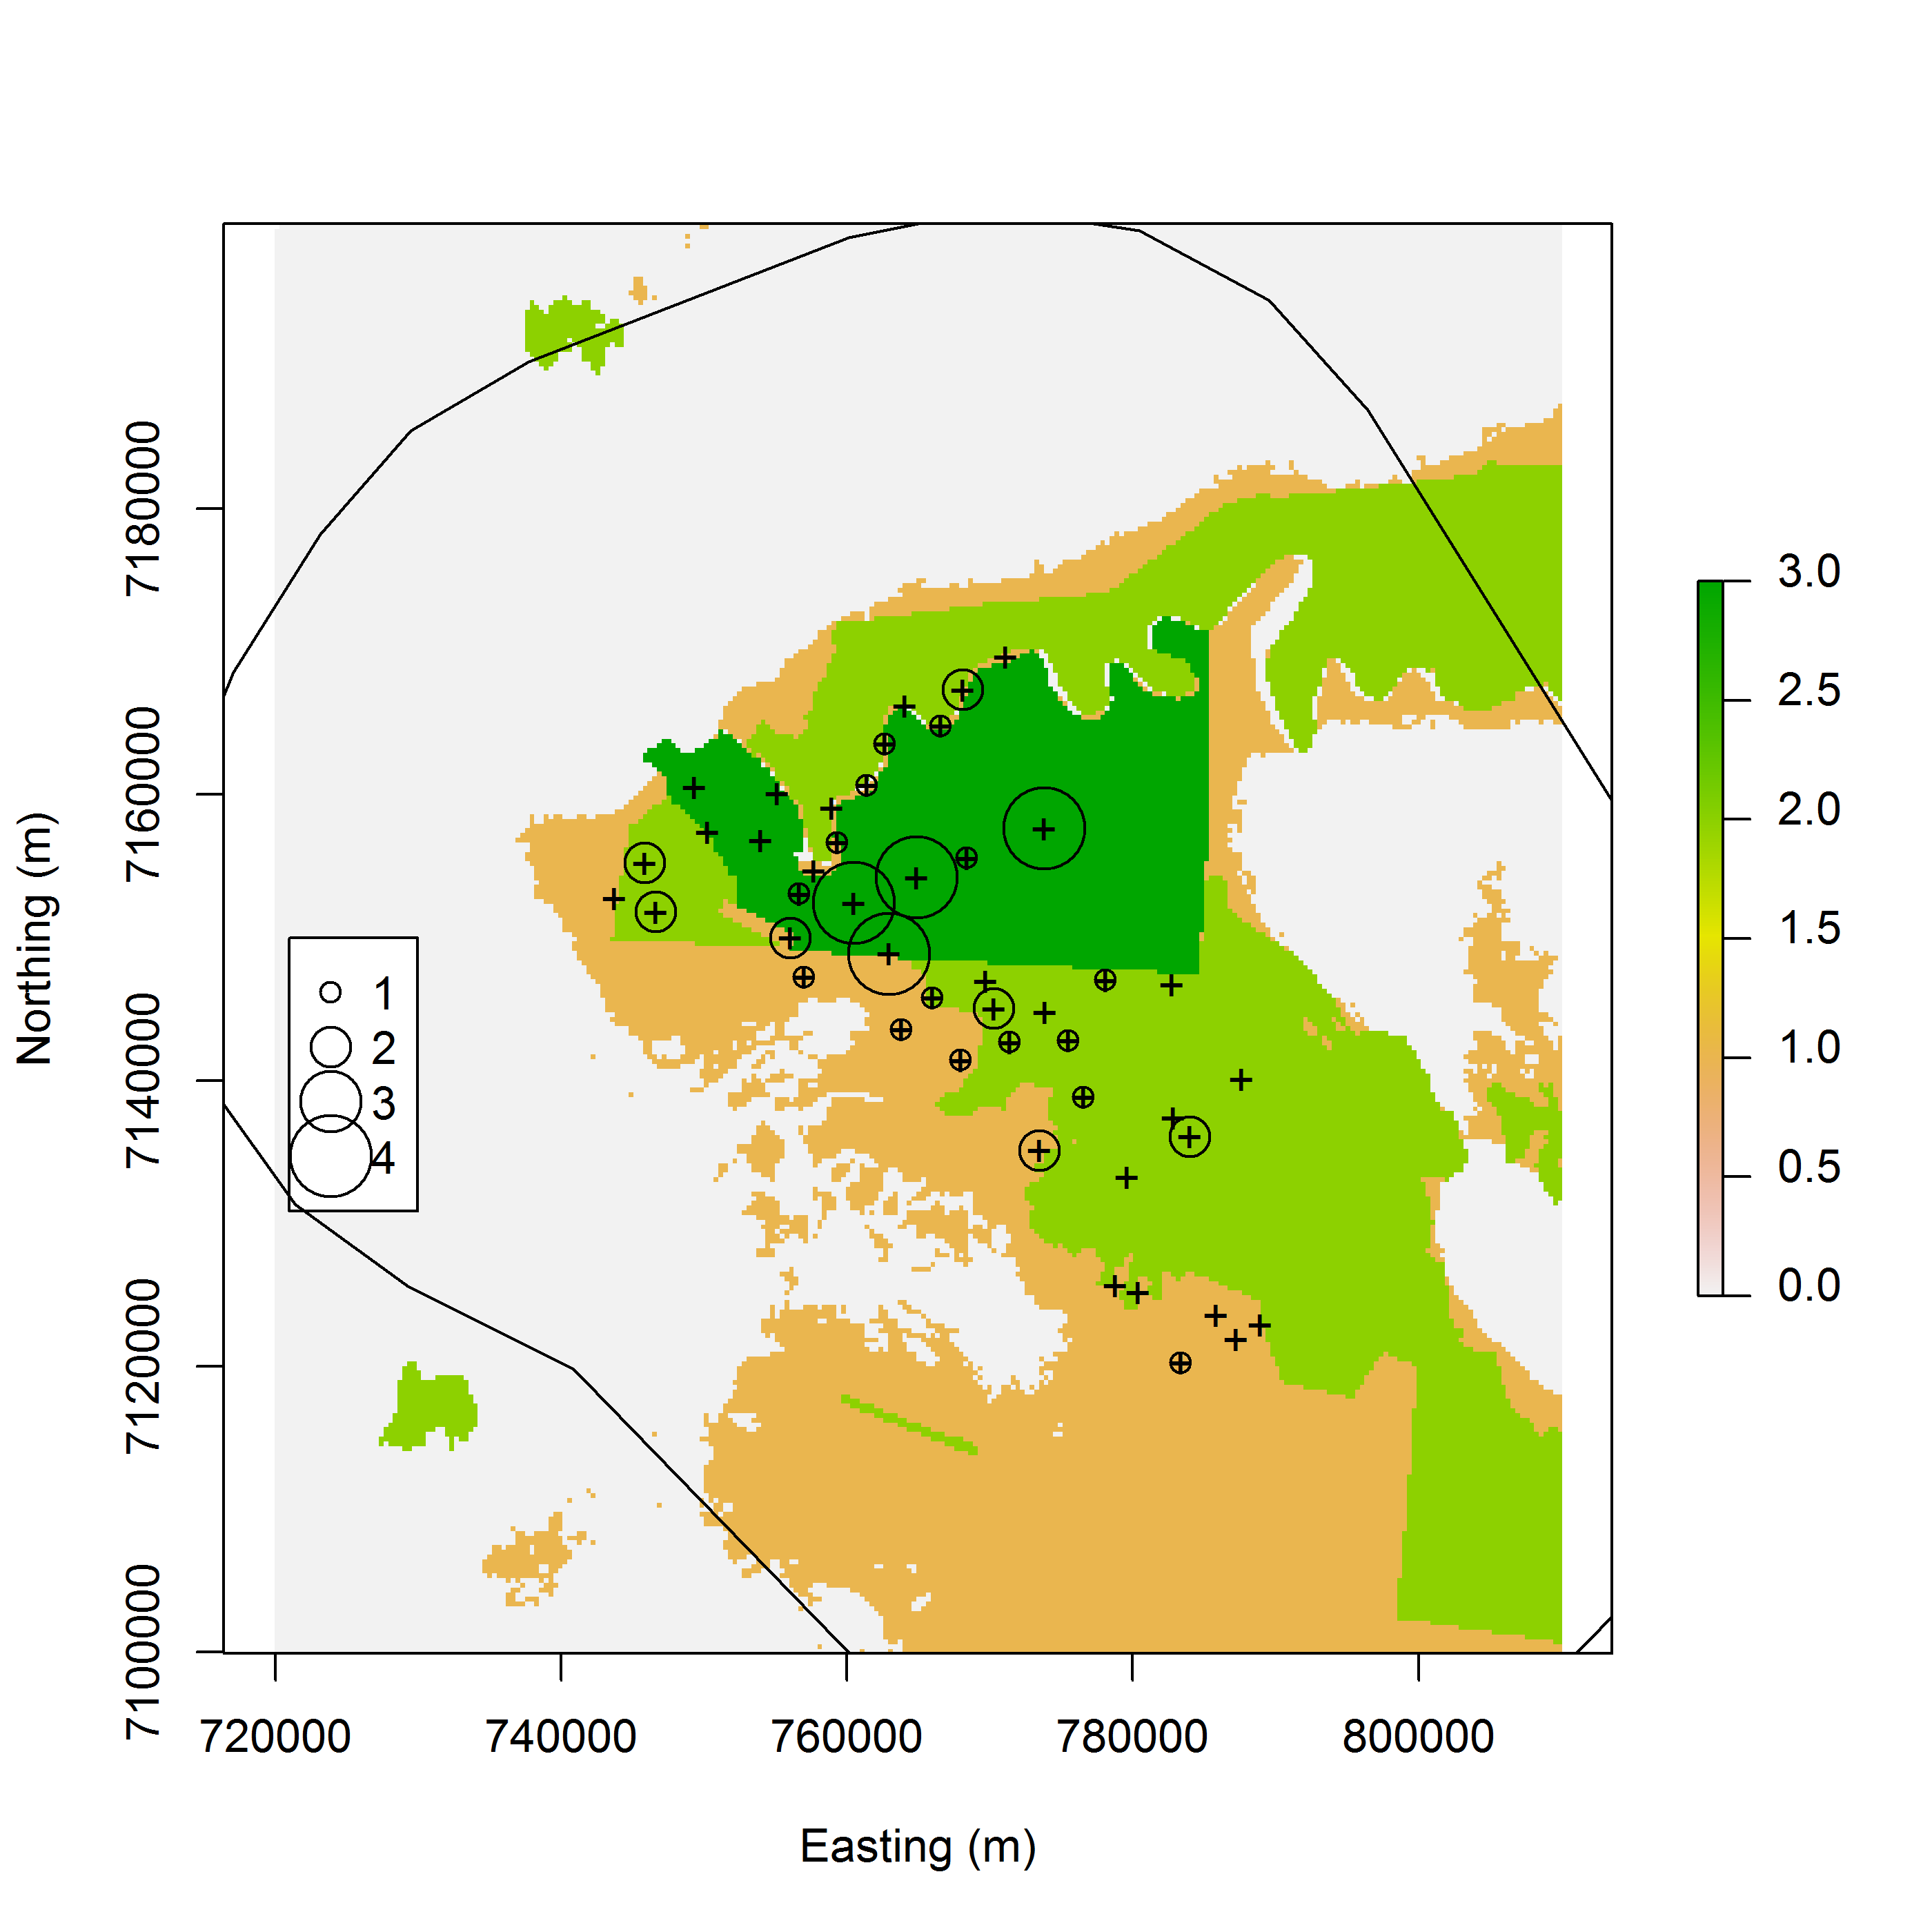
\includegraphics[width=3in,height=3in]{Ch11/figs/jaguarCountMap}
\label{ch9:fig:jaguarCts}
\caption{Jaguar detections at 46 camera trap stations. The three levels of
  protection status are no protection (beige), some protection (light
  green), and national park (dark green). Non-habitat is shown in gray
  and represents large soybean monocultures. }
\end{figure}

To assess the influence of protection on jaguar density, we treated
protection status as an ordinal variable with 3 levels: no protection,
some protection???, national park. Clearly these are ordered, and our
hypothesis is that density should increase with the level of
protection. Thus, $\bf \beta$ in this example is a single ``slope''
parameter describing the degree to which protection status affects
jaguar density. \r~code to fit the model are available in
\scrbook. Parameter estimates are shown in Table XXX. Our results
indicate that efforts to protect jaguars by reducing poaching are
working. Density was X times higher in the national park than in the
unprotected areas. Fig.~\ref{ch9:fig:Dsurface} shows the estimated
density surface.


\begin{table}
\caption{"Jaguar density estimates and associated parameters"}
\begin{tabular}{lrrrrr}
\hline
& Mean & SD & 2.5\% & 50\% & 97.5\% \\
 sigmaF &  7340.1547 &  1998.5926 &  4736.1803 &  6933.9760 & 12440.3079 \\
 sigmaM &  8154.5222 &  1581.5224 &  5801.0509 &  7916.7572 & 11890.7957 \\
 rho &     0.5163 &     0.1170 &     0.2874 &     0.5172 &     0.7388 \\
 lam0 &     0.0071 &     0.0024 &     0.0033 &     0.0067 &     0.0126 \\
 psi &     0.3145 &     0.0699 &     0.1908 &     0.3100 &     0.4638 \\
 beta &     4.3238 &     1.5115 &     2.4148 &     4.0295 &     8.0894 \\
 N &    20.3828 &     2.8671 &    16.0000 &    20.0000 &    27.0000 \\
 N1 &     0.2759 &     0.6360 &     0.0000 &     0.0000 &     2.0000 \\
 N2 &     2.6285 &     1.8589 &     0.0000 &     2.0000 &     7.0000 \\
 N3 &    17.4784 &     2.8458 &    12.0000 &    17.0000 &    24.0000 \\

\hline
\end{tabular}
\end{table}



\begin{figure}
\centering
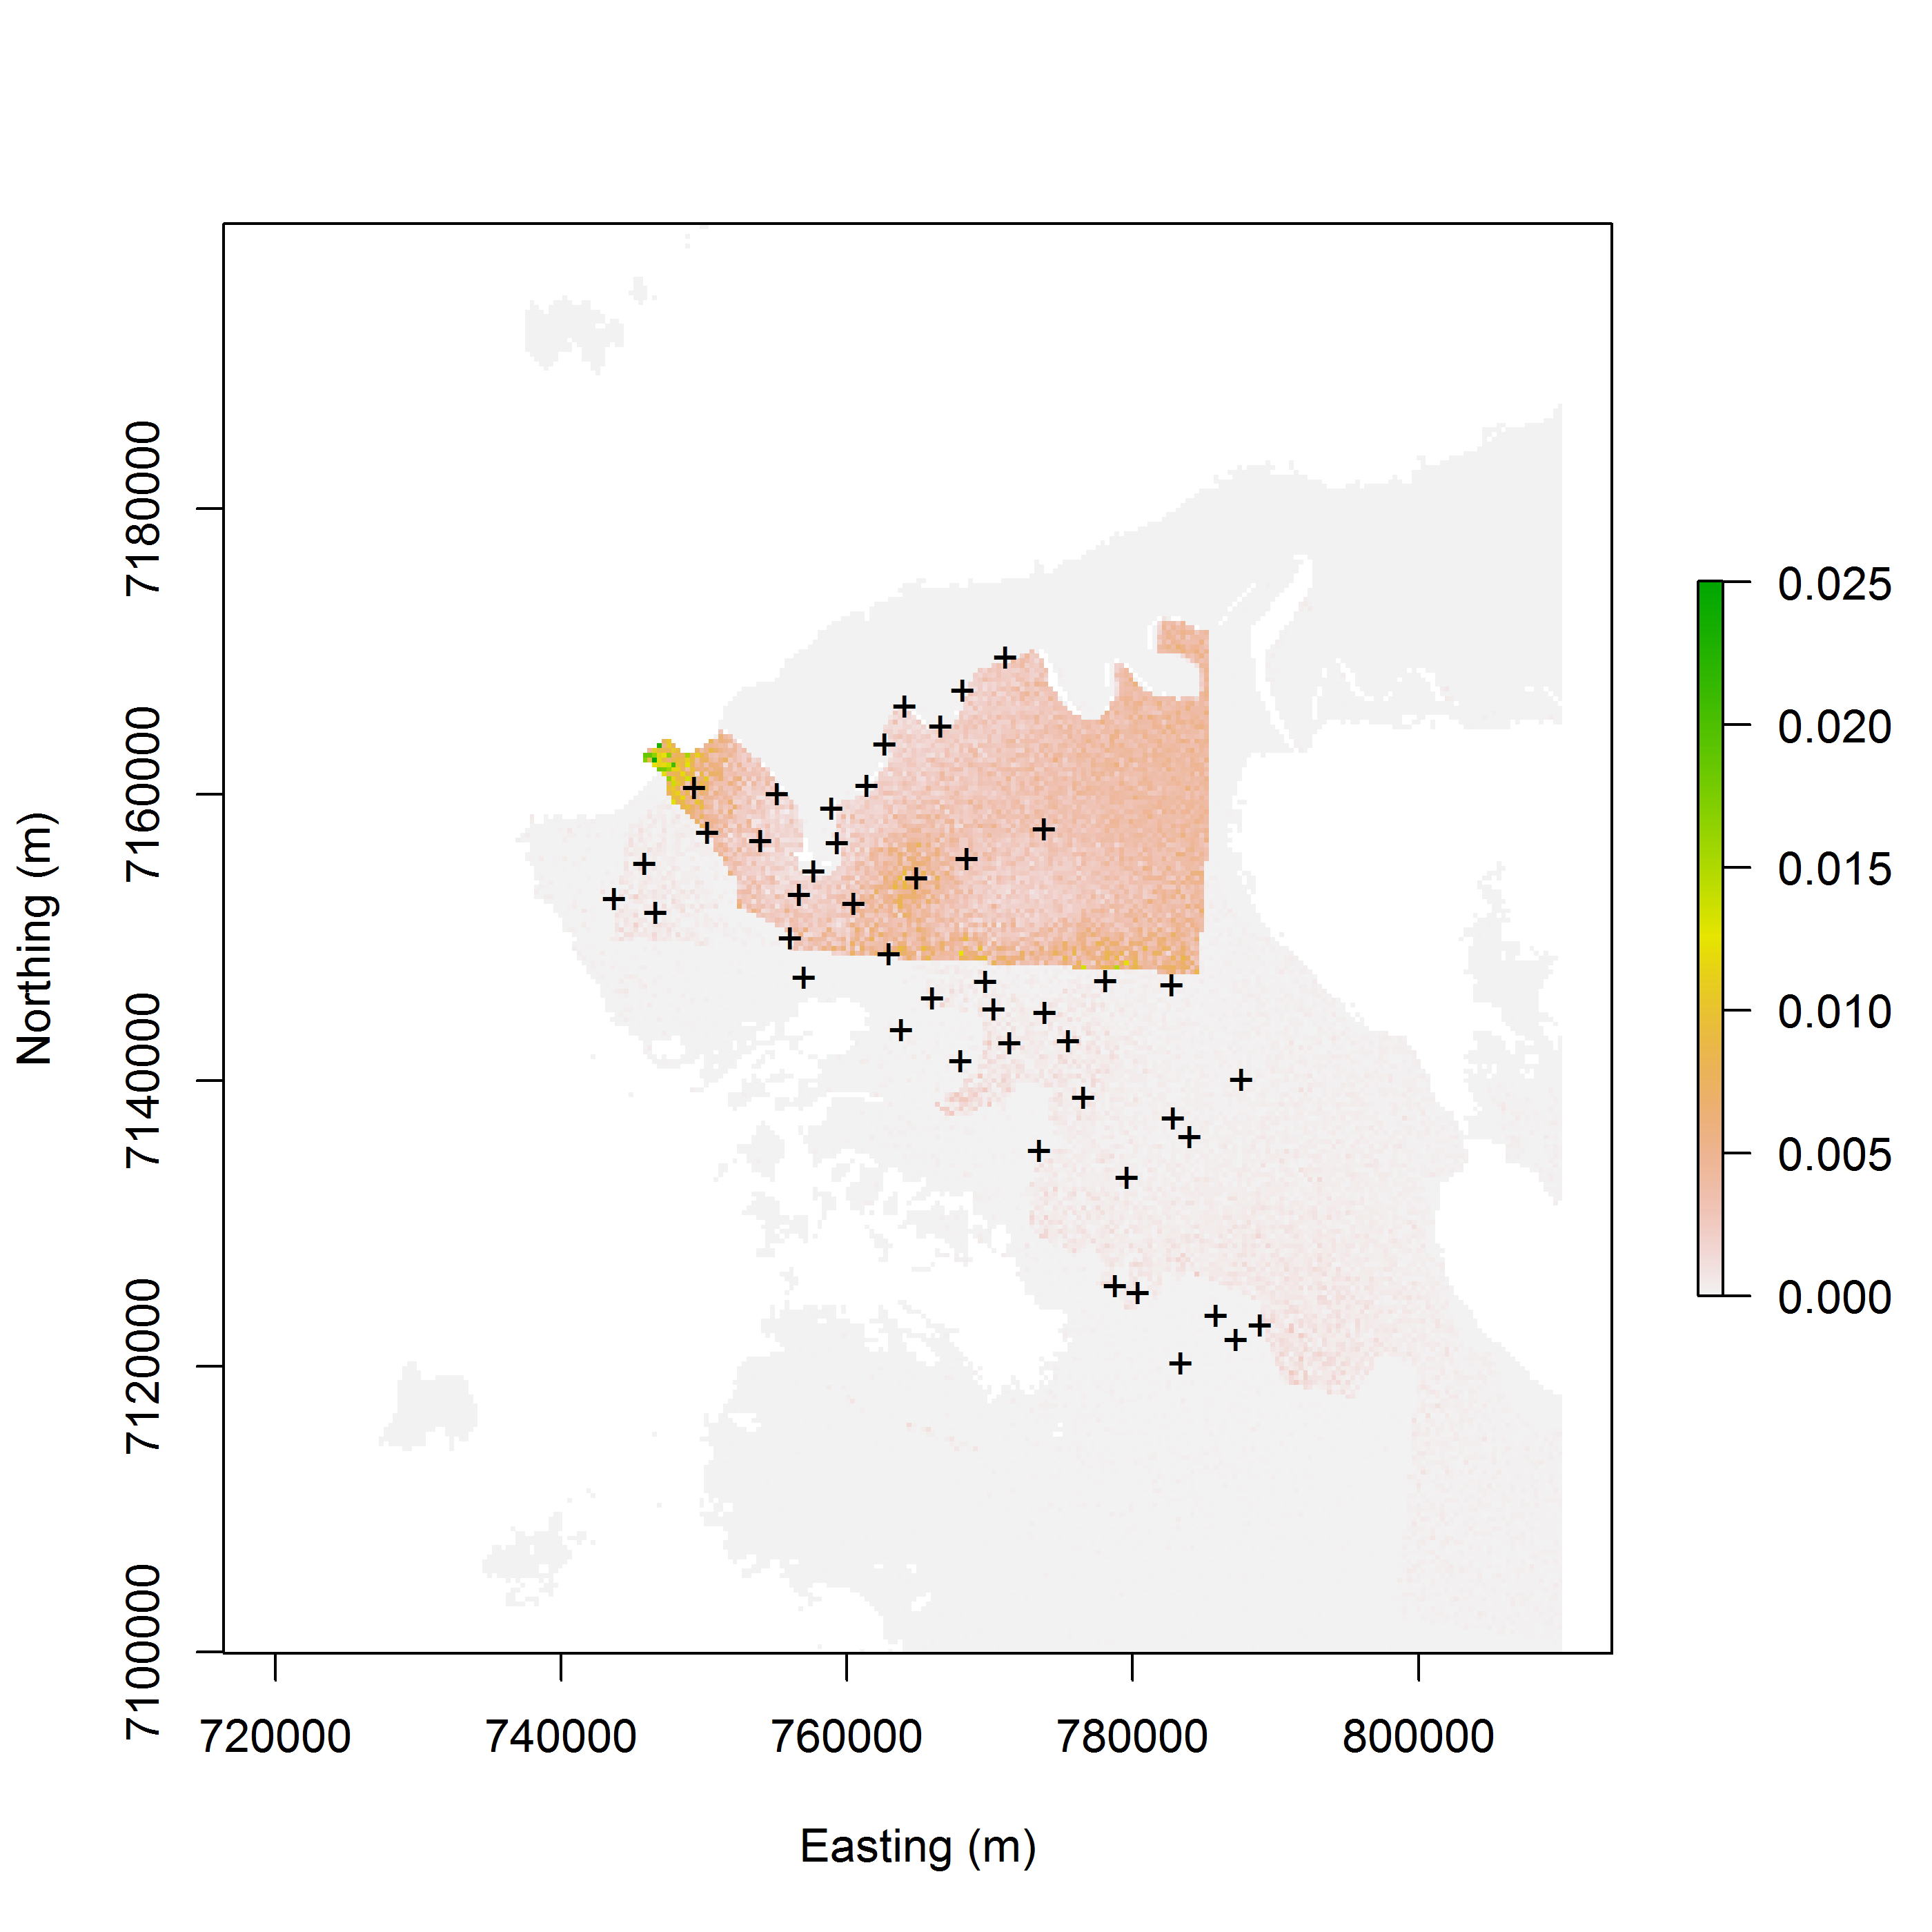
\includegraphics[width=3in,height=3in]{Ch11/figs/Dsurface34}
\label{ch9:fig:Dsurface}
\caption{Estimated density surface for the jaguar dataset}
\end{figure}

We note that there is room for improvement in our analysis. The
political boundaries use to demarcate protected areas are not as
concrete as we might like. In reality poaching pressure is likely to
be higher near remote park boundaries than in well-guarded park
interiors. One option
for addressing this would be to use a continuous measure of poaching
pressure such as distance from the nearest town, or some other
accessiblity metric. It would also be interesting to model density
seperately for each sex. Many of the detections outside of the park
were of males, and thus it is possible that the sexes use habitat
differently.




\section{Summary}

When state-space covariates are available, we can model
density by replacing the uniform prior on the activity centers with a
prior based on a normalized log-linear function of covariates. This
distribution has been widely used in ecology to model point processes
as well as resource selection probability functions. In our SCR
context, use of this new prior results in
a model for the inhomogeneous point process describing the
location of activity centers, which can be used to test hypotheses
about covariates affecting density. In
rare cases, these covariates are truly continuous in the sense that
they are defined as a function of space. More often, covariates are
represented on rasters, which simplifies the analysis. Fitting these
models can be accomplished using \bugs, \secr, or the custom \R~code
presented in this chapter and found in the package \scrbook.

Note that density cannot be modeled using traditional CR methods.

All the examples in this section included a single state-space
covariate, but this was for simplicity only. Including multiple
covariates poses no additional challenges. Likewise, additional model
structure such sex-specific encounter rate parameters or behavioral
responses can be accomodated.

